\chapter{System Design}

\section{Design Approach}

Function oriented design approach is comprised of many smaller sub-systems known as functions. These functions are capable of performing significant task in the system. The system is considered as top view of all functions.
Function oriented design inherits some properties of structured design where divide and conquer methodology is used.\\
This design mechanism divides the whole system into smaller functions, which provides means of abstraction by concealing the information and their operation. These functional modules can share information among themselves by means of information passing and using information available globally.\\
For this project, we are following a Function Oriented Design Approach. We have defined various functions depending upon our need. This way, we have complete control over different modules of our project. The main focus is on data. 




\section{System Design}
    \begin{itemize}
        \item \textbf{Acquiring Data}:- This part is concerned with acquiring data required for research work. The sources of this data can be data-set from Kaggle or from API.
        
        \item \textbf{Training Model}:- The model used in this research is trained using the data acquired in previous step. 
        
        \item \textbf{Long Short Team Memory Model}:- A deep learning model which uses historical data to train data set for predictive analysis i.e. prediction of time series data.
    \end{itemize} 

\newpage

\section{Workflow of Project}
\begin{figure}[ht]
    \centering 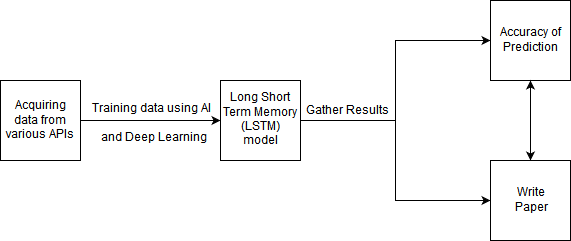
\includegraphics[scale=0.7]{images/fc.png}
    \caption{Workflow of Project}
\end{figure}


\section{Methodology}
    \begin{enumerate}
        \item \textbf{Acquiring Data}:- This part is concerned with acquiring data required for research work from various APIs. This data will be used for training model.
        
        \item \textbf{Long Short Team Memory Model}:- A deep learning model which will use acquired data and will generate the predicted values.

        \item \textbf{Accuracy of Prediction}:- Once the results are gathered, we need to check the accuracy of the gatherd results.
        
        \item \textbf{Writing Paper}:- Write and publish a Research Paper using the work done during the course of this project and the results obtained.
    \end{enumerate} 
